\chapter{Anwendung des Pointingmodells auf Daten des Teleskops}
\label{ch:auswertung}
Um das in Kapitel \ref{ch:pointing} entwickelte Pointingmodell zu testen, wurde mit dem Prototyp des MST ein Datensatz aufgenommen um 
\section{Datensatz}
\label{se:data}
Zur Analyse wurde der in der Nacht vom 4. auf den 5. Juli 2018 im Zeitraum von 21:00 UTC bis 1:45 UTC mit dem Prototypen des MST in Berlin-Adlershof aufgenommene Datensatz "run341" verwendet. Dazu wurden 105 Postionen (Abbildung \ref{img:record}) beobachtet, wobei das Teleskop anfangs Richtung Zenit stand und sich dann in einer abwärtslaufenden Spirale befand.
\begin{figure}[htbp]
\centering
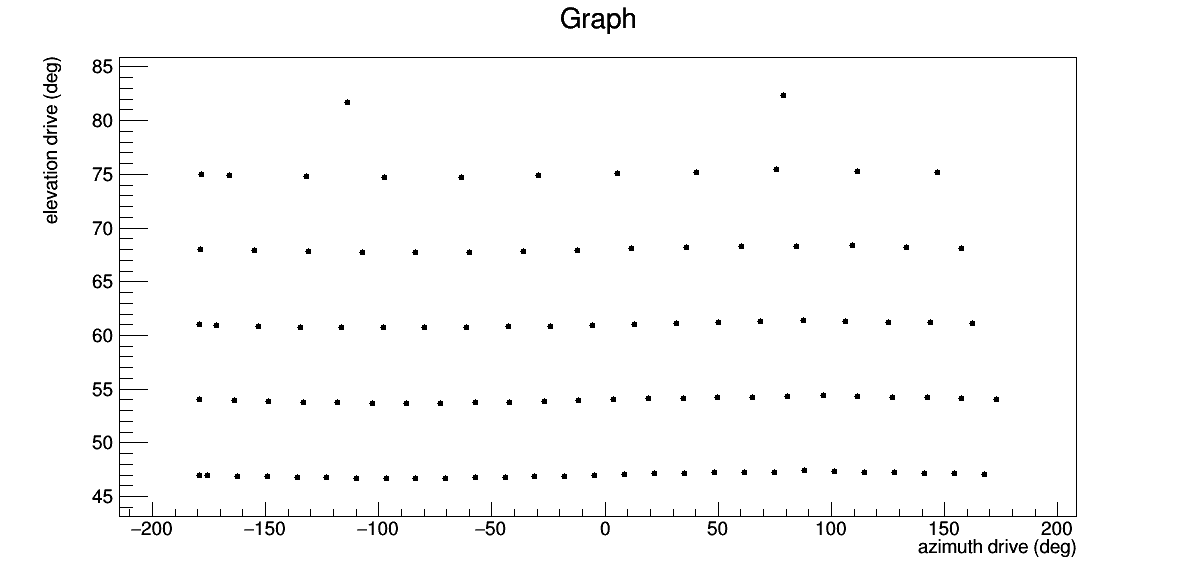
\includegraphics[width=\textwidth]{../341/data4.png}
\caption{Die am Teleskop eingestellten Position zur Datenaufnahme: Die Daten wurden in einer spiralförmigen Bewegung des Teleskops aufgenommen.}
\label{img:record}
\end{figure}
An jeder Position wurden 4 Bilder aufgezeichnet, wovon zwei eine Belichtungszeit von 20 Sekunden hatten.
Um die Bilder aufzunehmen, wurde eine Position des Nachthimmels eingestellt, die während der Belichtung des Bildes verfolgt wurde. Als Zeitstempel für die jeweiligen Bilder wird die Mitte der Belichtungszeit gewählt. Die jeweils zweiten Bilder werden hier zur Analyse verwendet. Dazu wird zunächst die Software \texttt{astrometry.net} verwendet, die aus den Bildern die jeweiligen Positionen der Sterne liest und diese mit dem bekannten Sternenhimmel vergleicht. Hierdurch lassen sich die Himmelskoordinaten des Mittelpunktes des Bildes sowie die Größe des Bildausschnittes bestimmen.
Die Himmelskoordinaten lassen sich mithilfe des Zeitstempels in das Koordinatensystem des Teleskops umrechnen und aus der Größe des Bildausschnitts lässt sich noch der Pixelscale bestimmen, der angibt, wie groß das Gesichtsfeld eines einzelnen Pixels ist. Da der Pixelscale kameraspezifisch und bekannt ist, lässt sich mit diesem überprüfen, ob das Bild richtig aufgelöst wurde. Von den 105 aufgenommenen Bildern konnten 100 gelöst werden, wobei der Pixelscale wie in Abbildung \ref{img:ps}
\begin{figure}[htbp]
\centering
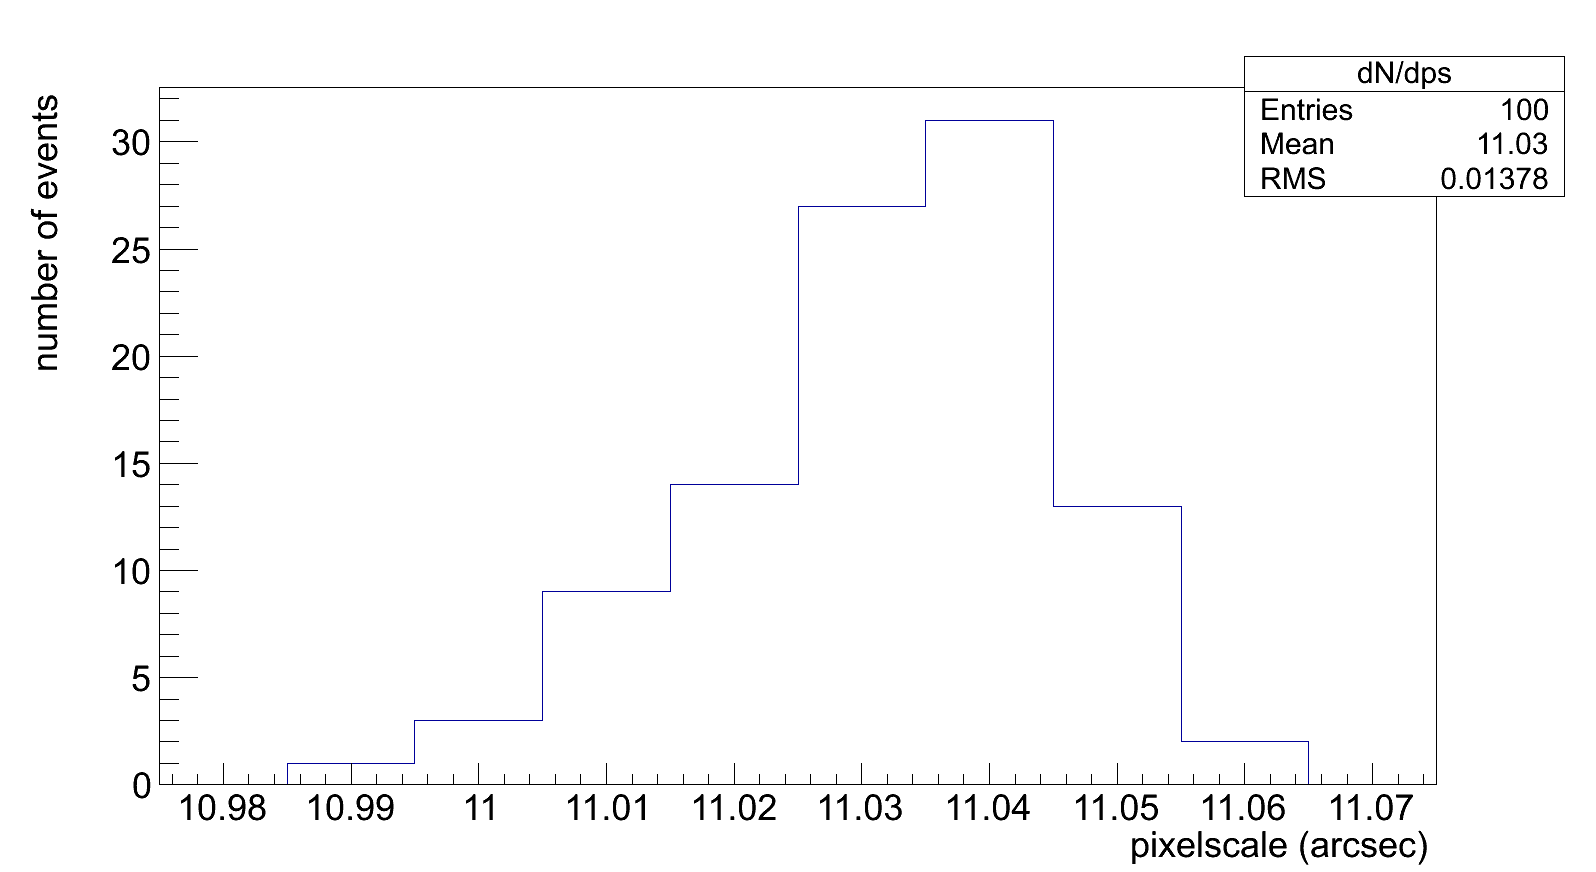
\includegraphics[width=\textwidth]{../341/histo.png}
\caption{Die Verteilung der von \texttt{astrometry.net} bestimmten Pixelscales: Diese sollte dem in Tabelle \ref{tab:SkyCCD} angegebenen Wert von $11.03\unit{arcsec}$ entsprechen.}
\label{img:ps}
\end{figure}
zu sehen ist, in keinem der Bilder um mehr als $0,04\unit{arcsec}$ abweicht. Somit können alle gelösten Aufnahmen zur Analyse verwendet werden. Die Differenzen zwischen Drive- und CCD-Koordinaten sind in \ref{img:dataset} dargestellt.
%\begin{figure}[htbp]
%\centering
%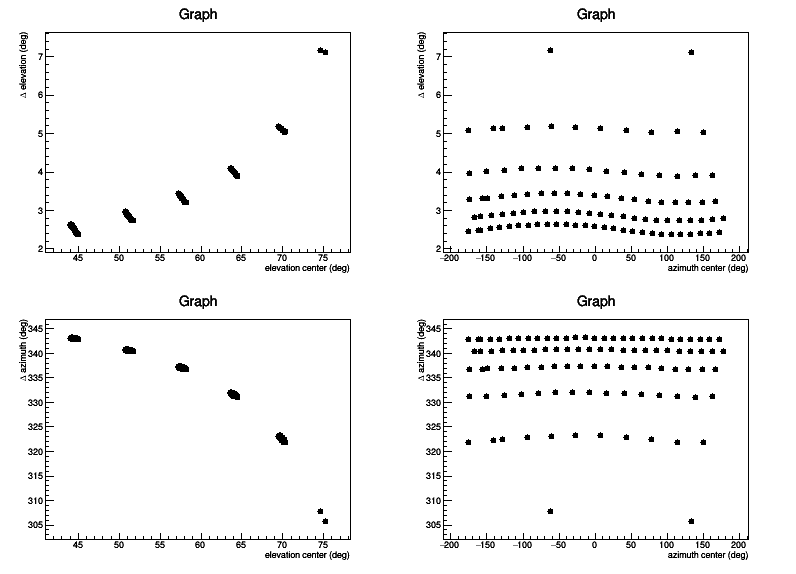
\includegraphics[width=\textwidth]{../341/data2.png}
%\label{img:dataset}
%\caption{Zu sehen sind die Differenzen (drive - CCD) in Abhängigkeit der von \texttt{astrometry.net} bestimmten Koordinaten für den Mittelpunkt der CCD-Aufnahmen}
%\end{figure}
\section{Bestimmung der optimalen Parameter für die Pointingmodelle}

Um das Pointingmodell auf Konsistenz zu überprüfen, wurde ein Programm mit \texttt{ROOT} geschrieben, das die optimalen Parameter für die in Kapitel \ref{ch:pointing} Pointingmodelle berechnet. Aus dem Vergleich der mit diesen Modellen vorhergesagten Werte mit den gemessenen Daten lassen sich dann Rückschlüsse über die Qualität der Pointingmodelle schließen. Um die optimalen Parameter zu berechnen werden zunächst die Abstände zwischen den vom Pointingmodell mit Parametern $\vec{q}$ bestimmten (Index P) und den experimentell bestimmten Positionen (Index E) bestimmt. Da alle Positionen, wie in Abbildung \ref{img:coordinates} zu sehen ist, auf einer Kugeloberfläche liegen, lässt sich der Abstand zwischen zwei Punkten durch einen Winkel 
\begin{equation}
\psi=\arccos\left(\sin(el_E)\sin(el_P)+\cos(el_P)\cos(el_E)\cos(az_P-az_E)\right).
\end{equation}
ausdrücken. Diese Winkelabstände werden für alle Wertepaare berechnet und summiert. Da die Winkel $\psi$ alle positiv sind, müssen hier keine Quadrate gebildet werden, wodurch die die Summe auch nicht durch Ausreißer dominiert wird. Die besten Parameter erhält man, wenn man die Summe der Winkelabstände minimiert. Dazu wird die Funktion \texttt{TMiniuit} verwendet. Um ein Maß für Güte des Modells zu bekommen wird die Größe $\frac{\chi^2}{doF}$ verwendet, die sich aus 
\begin{equation}
\chi^2=\sum^N_{i=1}\frac{\psi^2}{\sigma_i^2}
\end{equation}
und der Anzahl der Freiheitsgrade
\begin{equation}
doF=N-\textrm{Anzahl der Parameter}
\end{equation}
berechnet. Mit dem Wissen, dass der perfekte Wert für für $\frac{\chi^2}{doF}=1$ ist und der Annahme, dass alle Fehler gleich groß sind, lassen sich die Fehler wie folgt berechnen
\begin{equation}
\sigma=\sqrt{\frac{\sum^N_{i=1}\psi^2}{doF}}.
\end{equation}
Der $\chi^2$-Test ist in diesem Modell nur bedingt anwendbar, da bereits bekannt ist, dass das Teleskop noch weitere Fehler besitzt und das Modell somit auch nicht perfekt zu den Daten passen kann. Dennoch kann man so die Qualität des Modells beurteilen.\\
Zudem werden noch die Eigenschaften der Parameter bestimmt. Dazu wird ebenfalls mithilfe des \texttt{TMinuit}-Pakets die Kovarianzmatrix berechnet, die die Werte
\begin{equation}
COV(X,Y)=\left<\left(X-\left<X\right>\right)\cdot\left(Y-\left<Y\right>\right)\right>
\end{equation}
enthält. Auf der Hauptdiagonale stehen die Varianzen
\begin{equation}
COV(X,X)=VAR(X)=\sigma_X^2
\end{equation}
Interessant ist es auch, sich die Korrelation der Parameter untereinander anzusehen. Dazu wird der Korrelationskoeffizient 
\begin{equation}
\rho_{XY}=\frac{COV(X,Y)}{\sigma_X\sigma_Y}
\end{equation}
verwendet. Für $\rho=0$ liegt keine Korrelation vor und für $\rho=\pm1$ eine positive beziehungsweise eine negative Korrelation.

%Um das Pointingmodell auf Konsistenz zu überprüfen wurde ein Programm in ROOT geschrieben, welches die Differenzen der vom Pointingmodell (Index P) bestimmten Werte mit den gemessenen (Index M) Werten berechnet und analysiert. Da die oben entwickelten Pointingmodelle noch freie Parameter haben, die vom Teleskop abhängen werden diese durch eine Regression der Daten bestimmt. Da das Pointingmodell aus zwei Funktionen besteht (jeweils eine für die Elevation und den Azimut), die jedoch von den gleichen Parametern abhängen, muss hier ein kombinierter Fit durchgeführt werden. Dazu wird eine Hilfsvariable eingeführt, die die Summe der Quadrate der Differenzen von Messwerten und vorhergesagten Werten für feste Werte der freien Parameter bestimmt.
%\begin{equation}
%Q=\sum^N_{i=1}\left(P_i-M_i\right)^2
%\end{equation}
%Durch die Bildung der Quadrate können sich Abweichungen nach oben und unten nicht gegenseitig kompensieren und die Hilfsvariable ist somit ein Maß für die Abweichung von Modell mit den gewählten Parametern und Messwerten. Die besten Parameter erhält man, indem man die Variable minimiert. Dazu wurde die in ROOT integrierte Funktion TMinuit verwendet, die zudem noch die Standardabweichung der Parameter ausgibt. Um die Güte des Modells bestimmen zu können wird noch die Größe $\frac{\chi^2}{doF}$ verwendet um die Fehler der Messwerte zu bestimmen, in denen das Modell mit dem Datensatz übereinstimmt. Die Größe $\frac{\chi^2}{doF}$ ist definiert als
%\begin{equation}
%\frac{\chi^2}{doF}=\sum^N_{i=1}\frac{\left(P_i-M_i\right)^2}{\sigma_i^2}
%\end{equation}
%wobei hier $\sigma_i$ der Fehler des Wertes i ist und $doF$ der Anzahl der Freiheitsgraden entspricht. Diese berechnet sich durch
%\begin{equation}
%doF=N-\textrm{Anzahl der Parameter}
%\end{equation}
%Der perfekte Wert für $\frac{\chi^2}{doF}$ ist 1. Unter der Anahme, dass die Fehler $\sigma$ alle gleich groß sind, lassen sich diese wie folgt berechnen
%\begin{equation}
%\sigma=\sqrt{\frac{\sum^N_{i=1}\left(P_i-M_i\right)^2}{doF}}=\sqrt{\frac{Q}{doF}}
%\end{equation}
%Interessant ist es auch, sich die Korrelation der Parameter untereinander anzugucken. Die Korrelation beschreibt die Beziehung der zwischen einzelnen Parametern. Hier wird dazu der Korrelationskoeffizient nach Pearson verwendet, der ausschließlich die lineare Korrelation berücksichtigt. Um diesen zu berechnen wird zunächst die Korelationsmatrix
%\begin{equation}
%COV(X,Y)=\left<\left(X-\left<X\right>\right)\cdot\left(Y-\left<Y\right>\right)\right>
%\end{equation}
%berechnet. Auf der Hauptdiagonale stehen die Varianzen, aus denen sich die Fehler der Parameter bestimmen lassen:
%\begin{equation}
%\sigma_X=\sqrt{COV(X,X)}=\sqrt{VAR(X)}
%\end{equation}
%Der Korrelationskoeffizient lässt sich nun durch
%\begin{equation}
%\rho_{XY}=\frac{COV(X,Y)}{\sigma_X\sigma_Y}
%\end{equation}\\
%Um die Qualität der jeweiligen Pointingmodelle beurteilen zu können, werden jeweils vier Plots ausgegeben, die die jeweiligen Differenzen der bestimmten und gemessenen Koordinaten angeben
%\begin{equation}
%f=el_M-el_P \quad \textrm{bzw} \quad f=az_M-az_P
%\end{equation}
\section{Anwendung auf das Pointingmodell mit zwei Parametern}
Zunächst soll das in Kapitel \ref{ch:pointing} entwickelte Modell mit zwei Parametern, das einen konstanten Winkel zwischen der optischen Achse des Teleskops und der CCD-Kamera annimmt, untersucht werden.
\subsection{Abhängigkeit der Drivekoordinaten in Abhängigkeit der CCD-Koordinaten}
Begonnen wird mit der Vorhersage der Drive-Koordinaten mithilfe der CCD-Koordinaten. Unter der Annahme des festen Winkels zwischen Drive und Kamera wurden in Kapitel \ref{ch:pointing} die Abhängigkeiten aus den Formeln \ref{eq:elC2D} und \ref{eq:azC2D} vorhergesagt. Verwendet man das oben beschriebene Programm, erhält man die Parameter aus Tabelle \ref{tab:C2D}.
\begin{table}[htbp]
\centering
\begin{tabular}{rcl}
\toprule
$el_0$ &=& $(-1,20\pm0,57)^{\circ}$\\
$az_0$ &=& $(12,04\pm0,53)^{\circ}$\\
\bottomrule
\end{tabular}
\caption{Die beiden Parameter für die Vorhersage der Drivekoordinaten in Abhängigkeit der CCD-Koordinaten}
\label{tab:C2D}
\end{table}
Vergleicht man die Differenzen zwischen Drive- und CCD-Koordinaten mit den Differenzen zwischen Drive und den durch das Modell mithlife der CCD-Koordinaten vorhergesagten Koordinaten (gezeigt in Abbildung \ref{img:C2Dcomp}) so sieht man, dass das Modell die Abweichungen größtenteils kompensiert.
\begin{figure}[htbp]
\centering
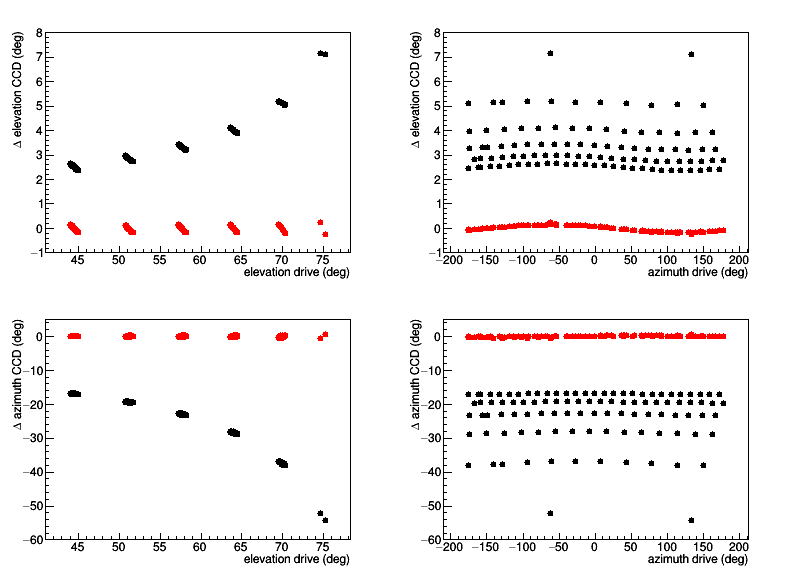
\includegraphics[width=\textwidth]{../341/C2Dcomp.png}
\caption{Die Abweichungen der mithilfe von zwei Parametern vorhergesagten CCD-Koordinaten zu den realen Werten (rot) im Vergleich zu den Differenzen zwischen Drive und CCD (schwarz): Das Modell eliminiert einen großen Teil der Abweichungen}
\label{img:C2Dcomp}
\end{figure}
Betrachtet man nur die Differenzen zwischen Pointingmodell und gemessenen Werten (Abbildung \ref{img:C2D}), so sieht man, dass die Werte noch von Null verschieden sind.
\begin{figure}[htbp]
\centering
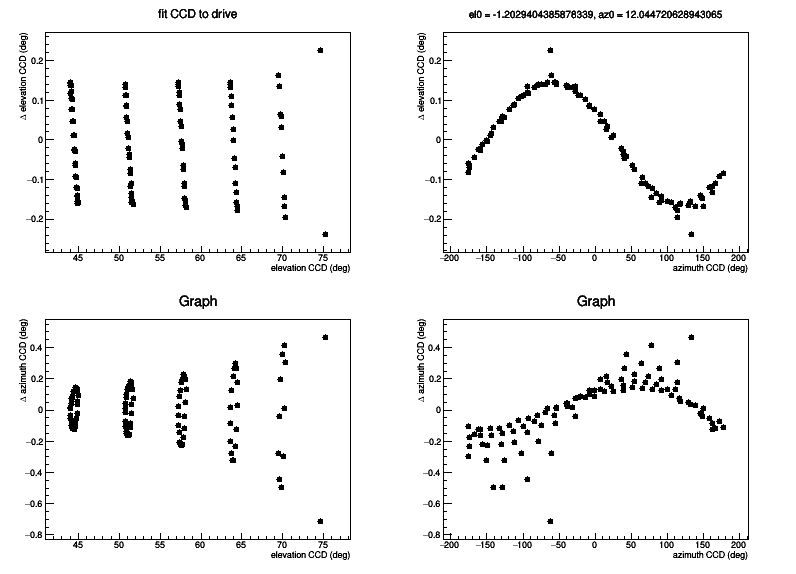
\includegraphics[width=\textwidth]{../341/C2D.png}
\caption{Die Abweichungen der vorhergesagten CCD-Koordinaten im Vergleich zu den gemessenen im Detail: Es sind noch systematische Abweichungen zu sehen, die darauf schließen lassen, dass das Modell noch nicht vollständig ist.}
\label{img:C2D}
\end{figure}
Das liegt nicht an ungenau bestimmten Werten, sondern hat, wie man besonders in den Graphen der Azimutabhängigkeit sehen, systematische Gründe. Solche Abweichungen waren durchaus zu erwarten, da das verwendete Pointingmodell nur den Fehler des konstanten Winkel zwischen der CCD-Kamera und der optischen Achse des Teleskops berücksichtigt. Zuletzt soll noch ein Graph (Abbildung \ref{img:C2Dcomp2}) betrachtet werden, der die vorhergesagten Koordinaten im Vergleich zu den gemessenen Koordinaten zeigt.
\begin{figure}[htbp]
\centering
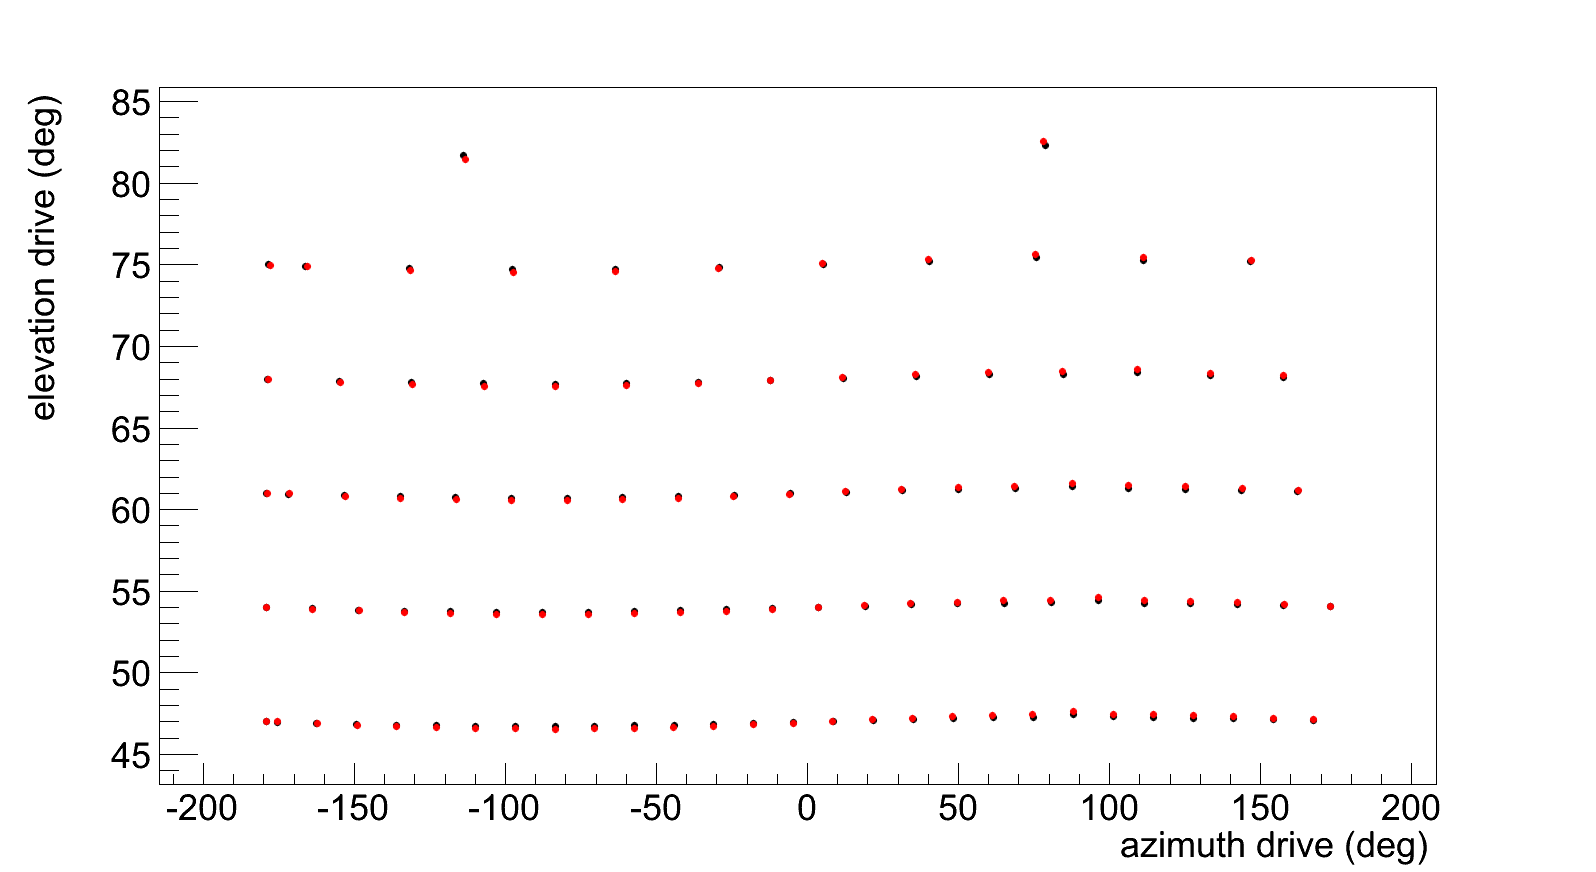
\includegraphics[width=\textwidth]{../341/C2Dcomp2.png}
\caption{Die vom Zwei-Parameter-Modell vorhergesagten Drive-Koordinaten (rot) im Vergleich zu den experimentell bestimmten (schwarz)}
\label{img:C2Dcomp2}
\end{figure}

\subsection{Abhängigkeit der CCD-Koordinaten in Abhängigkeit der Drivekoordinaten}
Möchte man jedoch die Koordinaten des Drives in Abbhängigkeit der CCD bestimmem, so benötigt man das inverse Modell, welches durch die Formeln \ref{eq:elD2C} und \ref{eq:azD2C} beschrieben wird. Für dieses Modell werden mithlife des Programms die Parameter in Tabelle \ref{tab:D2C} bestimmt.
\begin{table}[htbp]
\centering
\begin{tabular}{rcl}
\toprule
$el0$ &=& $(-1,20\pm0,54)^{\circ}$\\
$az0$ &=& $(12,05\pm0,51)^{\circ}$\\
\bottomrule
\end{tabular}
\label{tab:D2C}
\caption{Die beiden Parameter für die Vorhersage der CCD-Koordinaten in Abhängigkeit der Drive-Koordinaten}
\label{tab:D2C}
\end{table}
Wie erwartet liegen diese Werte sehr dicht an denen des obigen Modells (Tabelle \ref{tab:C2D}). Wie in Abbildung \ref{img:D2Ccomp} zu sehen ist, werden auch die Abweichungen ähnlich gut eliminiert. 
\begin{figure}[htbp]
\centering
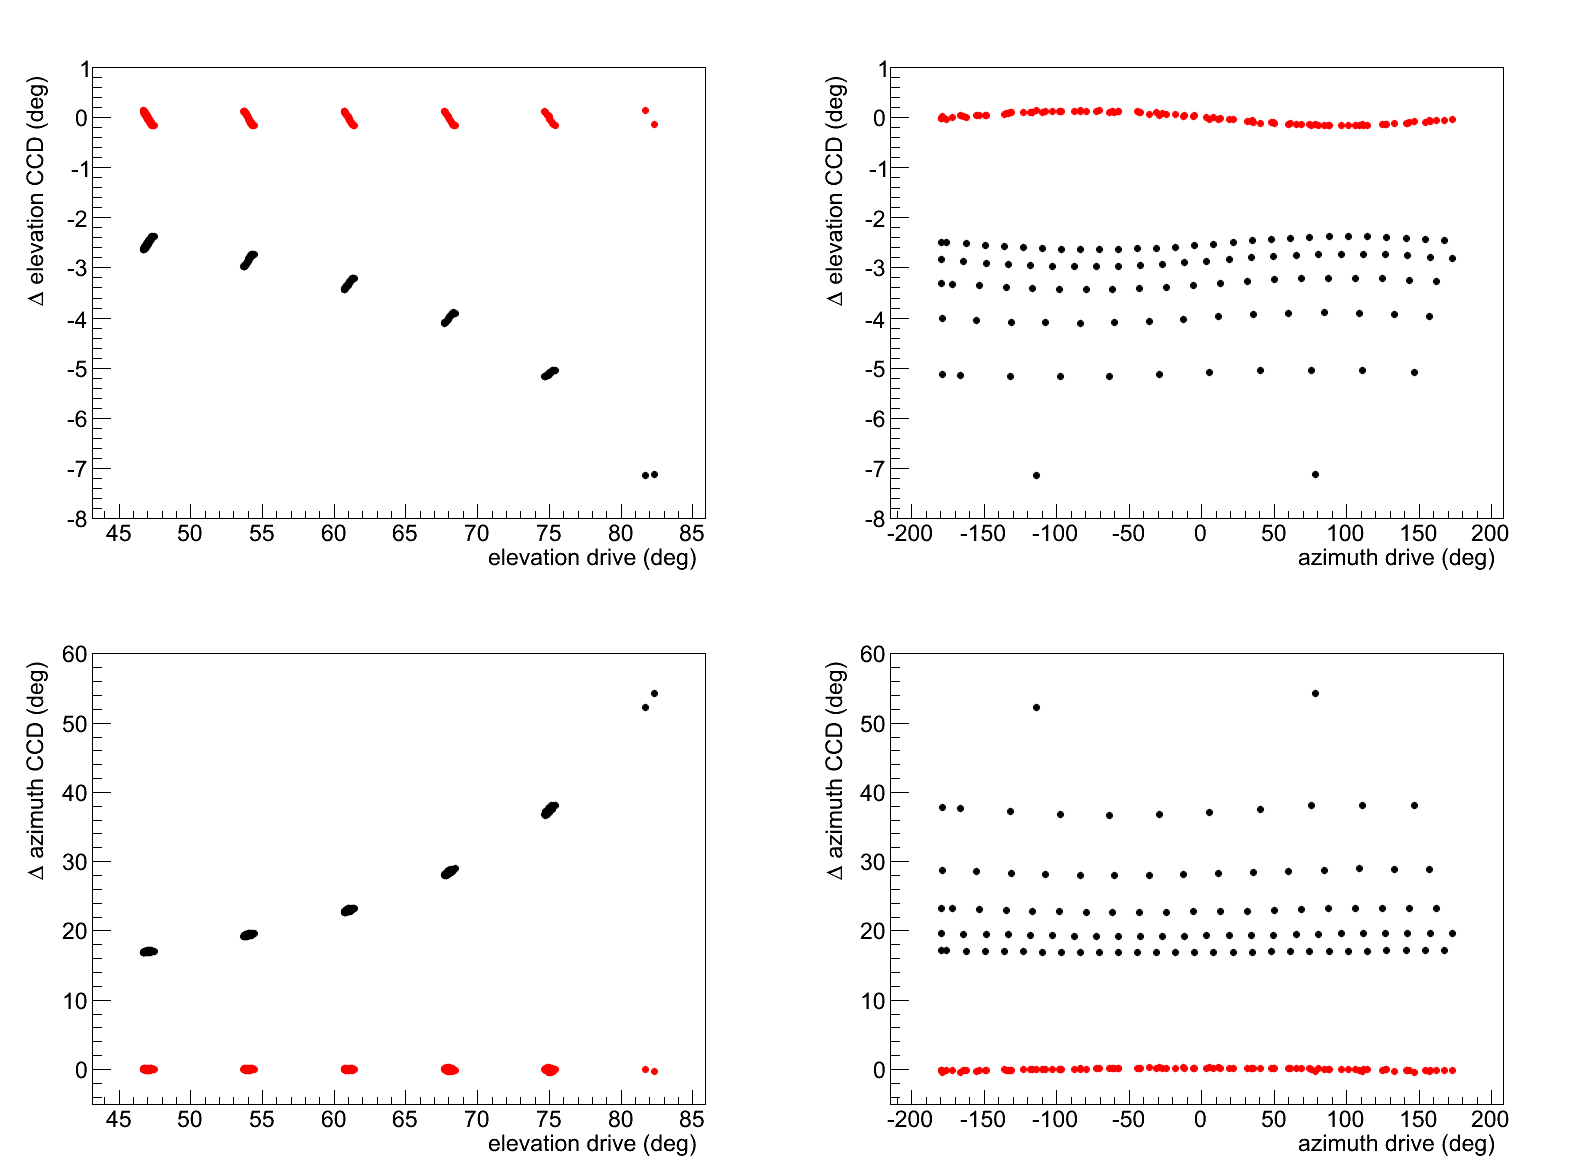
\includegraphics[width=\textwidth]{../341/D2Ccomp.png}
\caption{Die Abweichungen der vom Zwei-Parameter-Modell vorhergesagten CCD-Koordinaten zu den realen Werten (rot) im Vergleich zu den Differenzen zwischen Drive und CCD (schwarz): Wie beim inversen Modell werden die Abweichungen größtenteils korrigiert.}
\label{img:D2Ccomp}
\end{figure}
Betrachtet man wieder die Abweichungen des Pointingmodell isoliert (Abbildung \ref{img:D2C})
\begin{figure}[htbp]
\centering
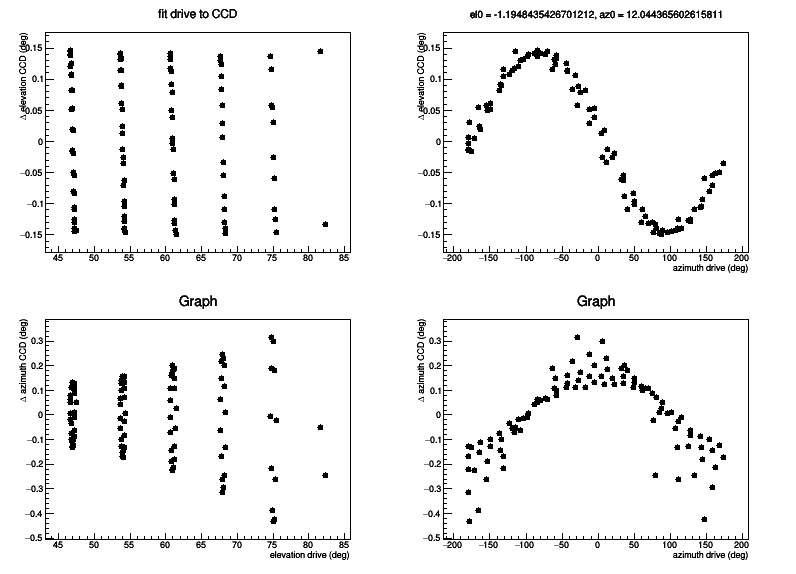
\includegraphics[width=\textwidth]{../341/D2C.png}
\caption{Gezeigt sind die Differenzen zwischen den vom Zwei-Parameter-Modell vorhergesagten CCD-Koordinaten und den gemessenen CCD-Koordinaten  im Detail: Hier sind ähnliche systematische Abweichungen wie im inversen Modell sichtbar.}
\label{img:D2C}
\end{figure}
so sieht man, dass für die beiden oberen Graphen die Effekte ähnlich wie die in Abbildung \ref{img:C2D} sind. Das die Graphen der Azimutabhängigkeit verzerrt aussehen, lässt sich durch den Wechsel der Koordinaten erklären.
\begin{figure}[htbp]
\centering
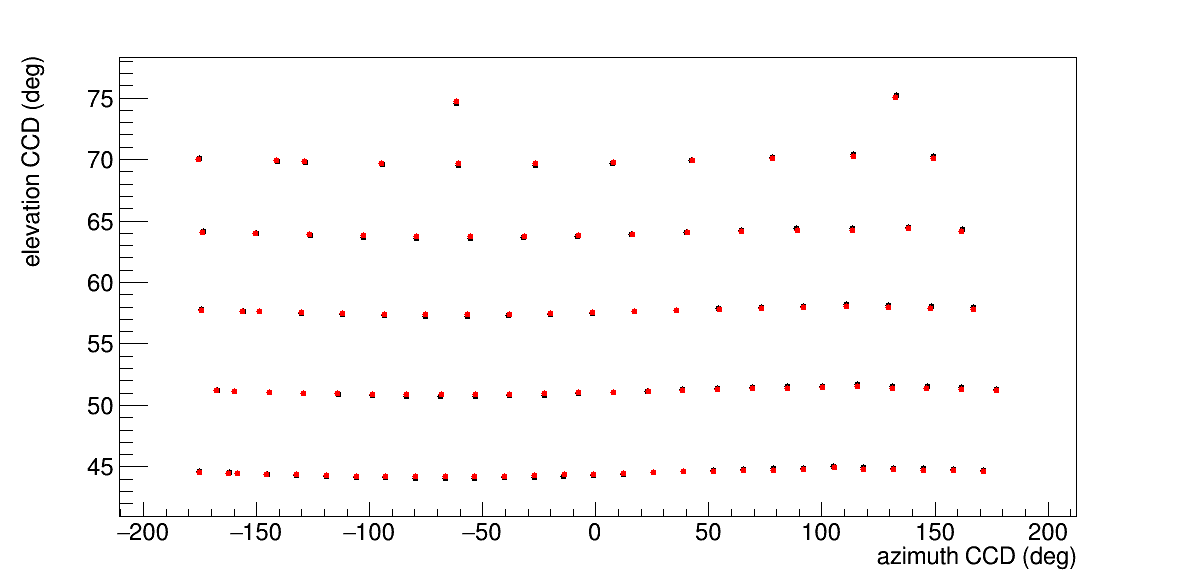
\includegraphics[width=\textwidth]{../341/D2Ccomp2.png}
\caption{Die vom Zwei-Parameter-Modell vorhergesagten CCD-Koordinaten (rot) im Vergleich zu den experimentell bestimmten (schwarz)}
\label{img:D2Ccomp2}
\end{figure}

\section{Anwendung auf das Pointingmodell mit 4 Parametern}
Im Folgenden wird das oben verwendete Modell erweitert, indem man wie in Abschnitt \ref{se:4par} annimmt, dass die eingestellten Koordinaten zu den tatsächlichen um jeweils einen konstanten Wert verschoben sind. Zu den obigen Parametern $el_0$ und $az_0$ kommen somit noch die Parameter $az_1$ für eine konstante Verschiebung im Azimut und $el_1$ für eine konstante Verschiebung in der Elevation hinzu.
\subsection{Abhängigkeit der Drivekoordinaten in Abhängigkeit der CCD-Koordinaten}
Hier wird wie oben mit der Vorhersage der Drive-Koordinaten in Abhängigkeit der CCD begonnen. Dazu verwendet man die Formeln \ref{eq:elC2D4} und \ref{eq:azC2D4}, für die sich mithilfe des Fit-Programms die Parameter aus Tabelle \ref{tab:C2D4} berechnen lassen.
\begin{table}[htbp]
\centering
\begin{tabular}{rcl}
\toprule
$el_0$ &=& $(-1,1\pm 4,9)^{\circ}$\\
$az_0$ &=& $(12,0\pm 3,6)^{\circ}$\\
$el_1$ &=& $(-0,14\pm 5,96)^{\circ}$\\
$az_1$ &=& $(0,03\pm 4,20)^{\circ}$\\
\bottomrule
\end{tabular}
\caption{Die vier Parameter um die CCD-Koordinaten durch das erweiterte Pointingmodell vorherzusagen}
\label{tab:C2D4}
\end{tabular}
\end{table}
Hier fällt auf, dass die Fehler im Gegensatz zum Zwei-Parameter-Modell deutlich größer geworden sind. Außerdem sind die Werte für die neu hinzugefügten Modelle zu vernachlässigen. Um zu überprüfen, inwiefern der zu den Drive-Koordinaten hinzugefügte Offset das Zwei-Parameter-Modell verbessert, werden zunächst die Abstände der beiden Modelle gemeinsam in Abbildung \ref{img:C2D4comp} dargestellt.
\begin{figure}[htbp]
\centering
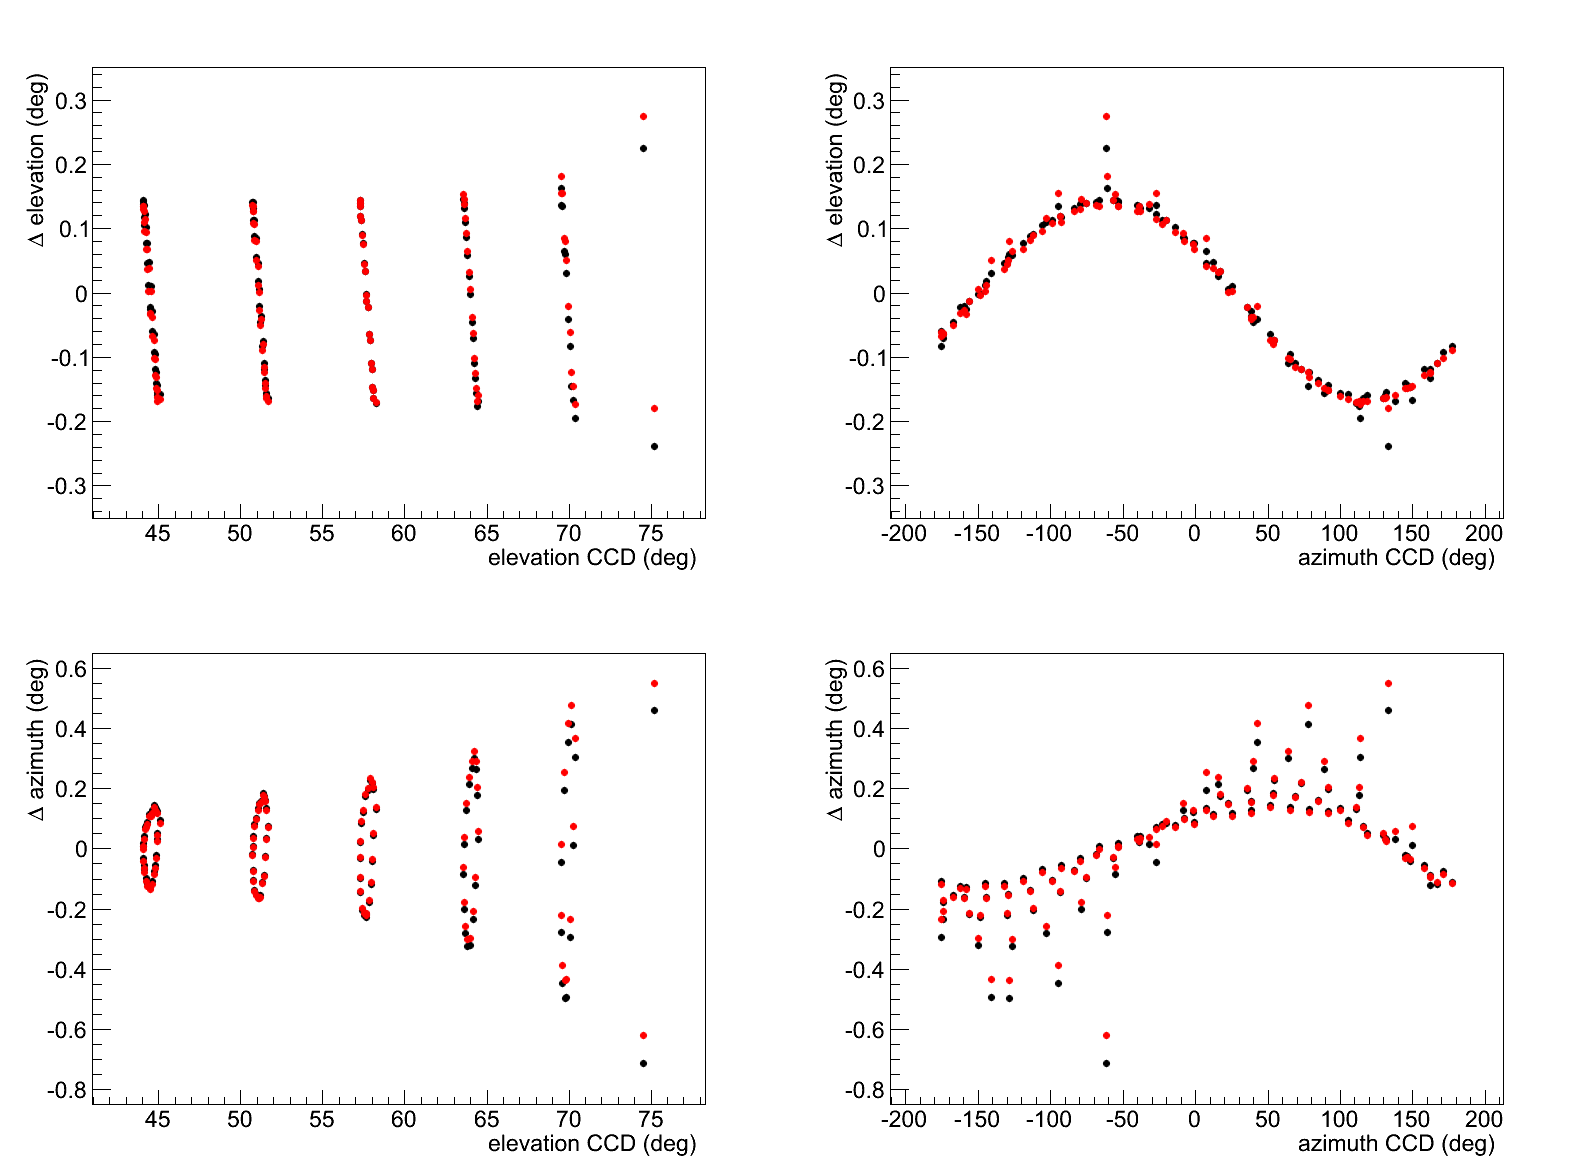
\includegraphics[width=\textwidth]{../341/C2D44comp.png}
\caption{Vergleich der Differenzen zwischen den vom Vier-Parameter-Modell (rot) bzw vom Zwei-Parameter-Modell (schwarz) vorhergesagten Drive-Koordinaten und den realen Werten: Die beiden zusätzlichen Parameter bringen kaum eine Verbesserung.}
\label{img:C2D4comp}
\end{figure}
In der Abbildung sind lediglich für große Elevationswerte des Drives Abweichungen zu erkennen. Aufgrund der kleinen Werte für die Parameter $az_1$ und $el_1$ sind zunächst keine großen Änderungen zum Zwei-Parameter-Modell zu erwarten. Zudem überwiegt beispielsweise im Graphen rechts oben eine Wellenbewegung, die sich nicht durch einen konstante Verschiebung korrigieren lässt. Vergleicht man die vorhergesagten Positionen mit den gemessenen Positionen (Abbildung \ref{img:C2D4comp2}) erhält man aufgrund der nur kleinen Korrekturen zum Zwei-Parametermodell ein ähnliches Verhalten wie in Abbildung \ref{img:C2Dcomp2}.
\begin{figure}[htbp]
\centering
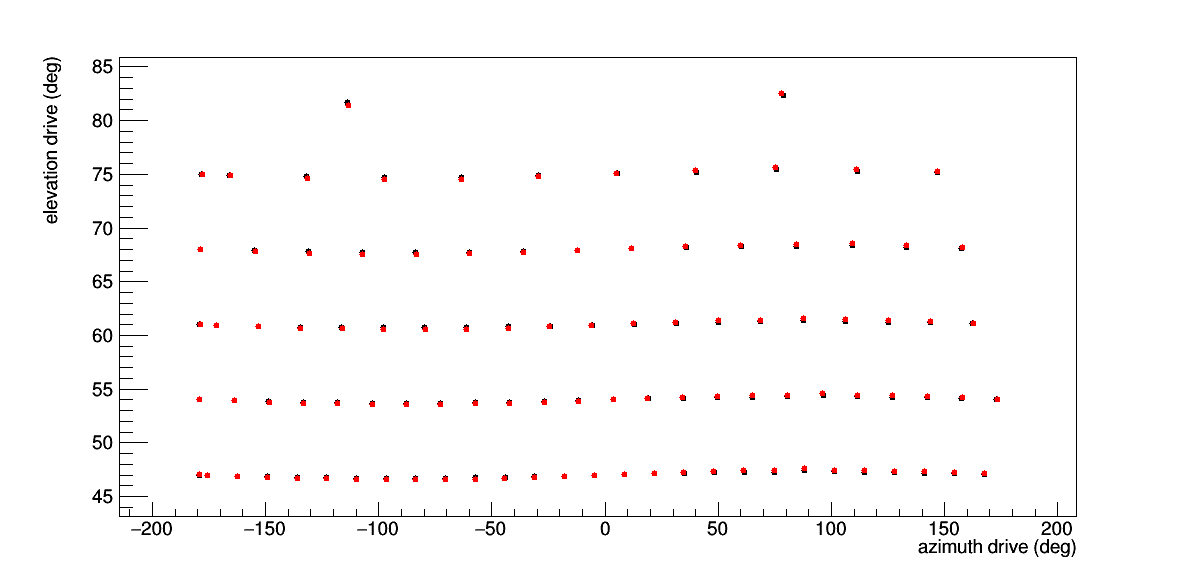
\includegraphics[width=\textwidth]{../341/C2D4comp2.png}
\caption{Die vom Vier-Parameter-Modell vorhergesagten Drive-Koordinaten (rot) im Vergleich zu den experimentell Bestimmten (schwarz): Es ist kaum ein Unterschied zum Zwei-Parameter-Modell zu erkennen.}
\label{img:C2D4comp2}
\end{figure}

\subsection{Abhängigkeit der CCD-Koordinaten in Abhängigkeit der Drivekoordinaten}
Zuletzt wird das Vier-Parameter-Modell benutzt um die CCD-Koordinaten durch die Drive-Koordinaten vorherzusagen. Dazu wird das im Vergleich zu oben invertierte Modell, welches durch die Gleichungen \ref{eq:elD2C4} und \ref{eq:azD2C4} beschrieben wird, verwendet. Für diese Formeln erhält man die in Tabelle \ref{tab:D2C4} stehenden Parameter.
\begin{table}[htbp]
\centering
\begin{tabular}{rcl}
\toprule
$el_0$ &=& $(-1,2\pm 77,52)^{\circ}$\\
$az_0$ &=& $(12,1\pm 2,1)^{\circ}$\\
$el_1$ &=& $(0,04\pm 79,29)^{\circ}$\\
$az_1$ &=& $(-0,06\pm 3,61)^{\circ}$\\
\bottomrule
\end{tabular}
\caption{Die für das Pointingmodell mit vier Parametern bestimmten Werte, wobei die CCD-Koordinaten in Abhängigkeit der Drive-Koordinaten vorhergesagt wurden.}
\label{tab:D2C4}
\end{table}
Im Vergleich zu den Parametern im inversen Modell sind hier die Fehler noch mal deutlich angestiegen. Der Grund hierfür ist die Korrelation der Parameter. Die Addition einer kleinen Konstanten zu einer Drehung verhält sich sehr ähnlich zur Summe dieser beiden Winkel. Die Fehler für $el_0$ und $ez_1$ sind beide ähnlich groß, was auf eine starke negative Korrelation schließen lässt. Tatsächlich wurde für diese beiden Parameter der Korrelationskoeffizient 
\begin{equation}
\rho_{el_0,el_1}= -0,9999
\end{equation}
ermittelt. Ähnlich sieht für die Korrelation zwischen $az_0$ und $el_0$ aus. Hier ist der Korrelationskoeffizient
\begin{equation}
\rho_{az_0,az_1}= -0,9526
\end{equation}
ähnlich groß. Da gerade in diesem Modell die Parameter sehr ähnlich zu denen des Zwei-Paramter-Modells sind (dort sind die zusätzlichen Paramter Null) erwartet man keine großen Unterschiede zwischen diesen Modellen. Diese These wird durch Abbildung \ref{img:D2C4comp} bestätigt.
\begin{figure}[htbp]
\centering
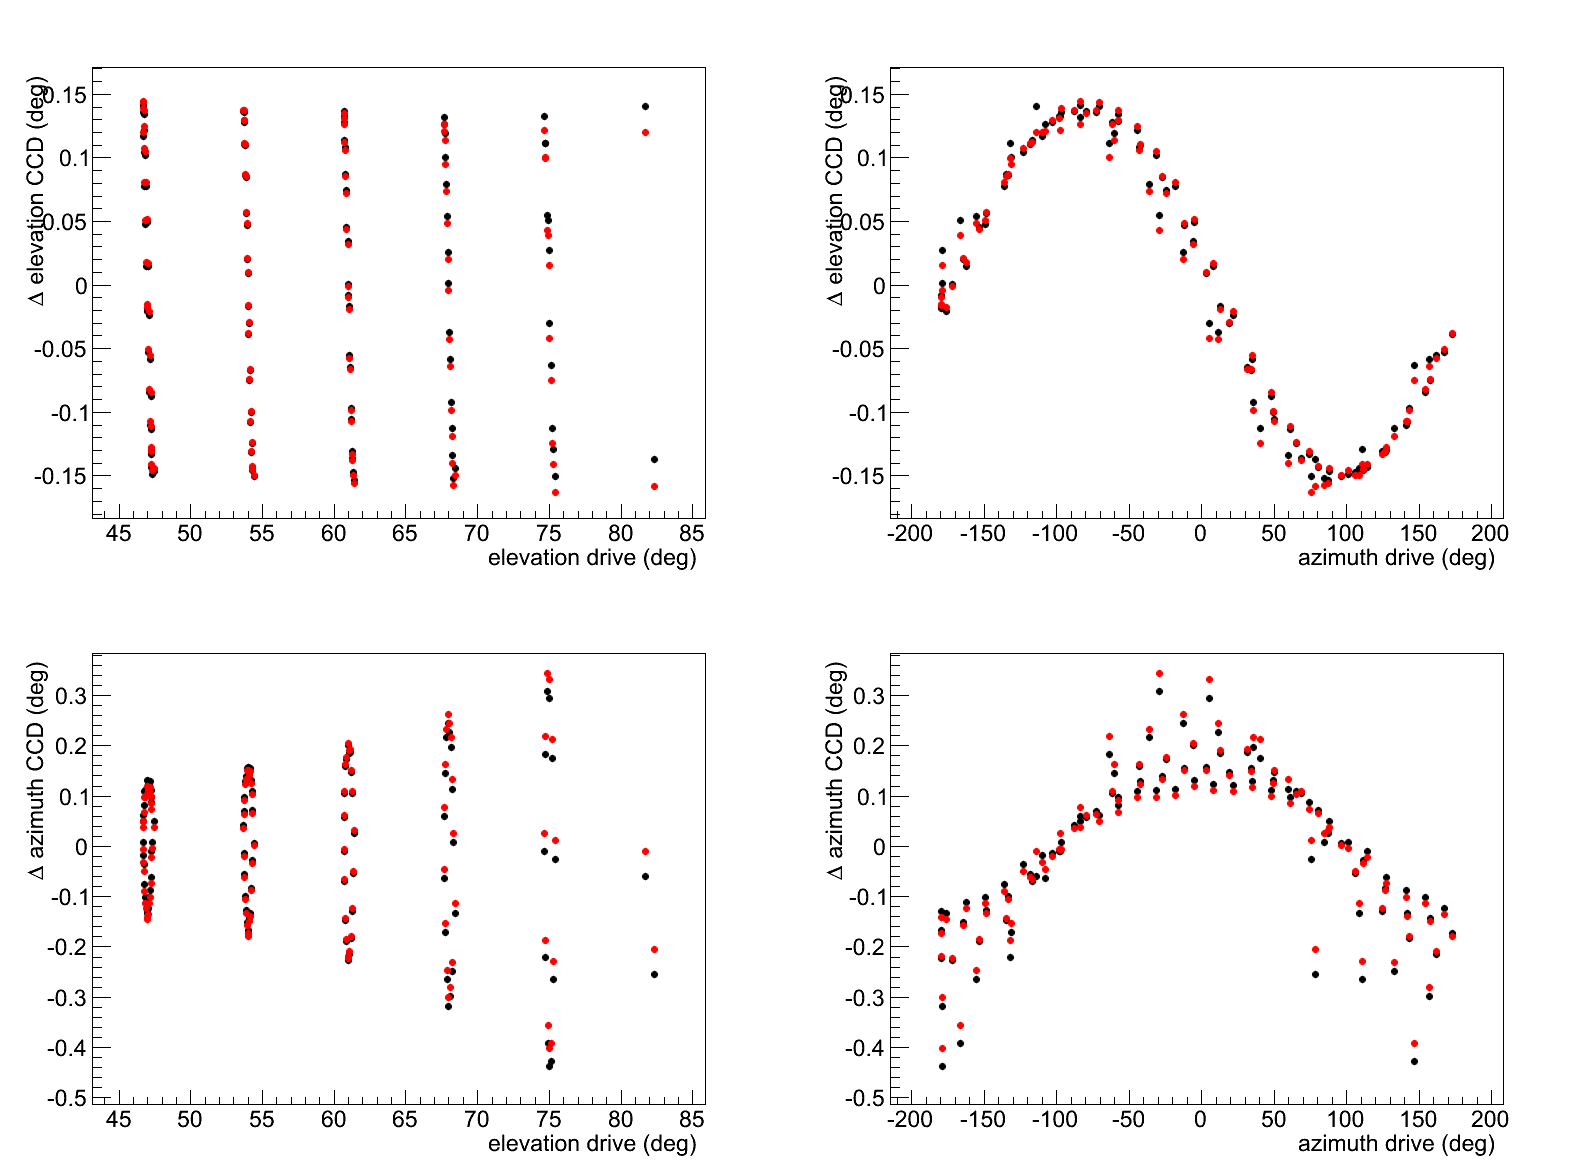
\includegraphics[width=\textwidth]{../341/D2C44comp.png}
\caption{Das Vier-Parameter-Modell (rot) für die Vorhersage der CCD-Koordinaten im Vergleich zum Zwei-Parameter-Modell (schwarz): Wie erwartet sind kaum Verbesserungen zu erkennnen.}
\label{img:D2C4comp}
\end{figure}
Somit gibt es auch keine nennenswerte Veränderung im Vergleich der vorhergesagten und experimentell bestimmten Positionen
\begin{figure}[htbp]
\centering
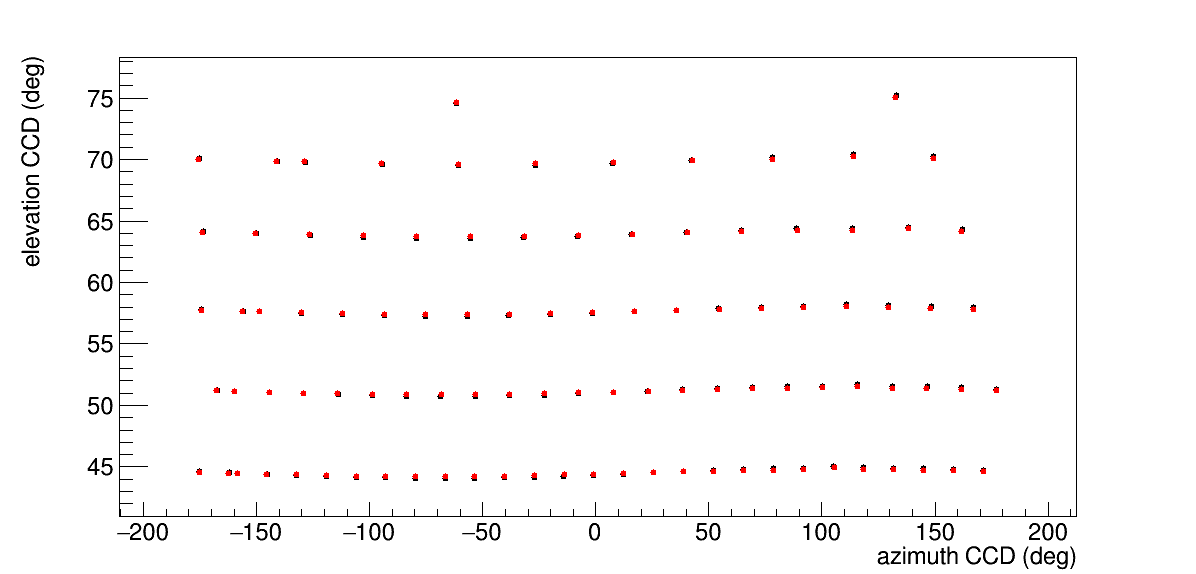
\includegraphics[width=\textwidth]{../341/D2C4comp2.png}
\caption{Die vom Vier-Parameter-Modell (rot)vorhergesagten Koordinaten der CCD im Vergleich zu den experimentell bestimmten.}
\label{img:D2C4comp2}
\end{figure}

\section{Systematische Abweichungen im entwickelten Pointingmodell}
Betrachtet man die Graphen der Differenzen, so erkennt man, dass noch weitere Effekte das Pointing erschweren. Zunächst wird das weitere Verhalten der Elevation betrachtet. Hier fällt bei der Betrachtung von $\Delta el$ in Abhängigkeit des Azimuts auf, dass der Graph eine Wellenbewegung beschreibt. Aus dem Graph, der die Elevationsabhängigkeit beschreibt, lässt sich hingegen keine keine systematische Abweichung erkennen. Ein solches Verhalten könnte beispielsweise die Verkippung der Turmachse erklären. Durch eine solche Verkippung zeigt die Kamera auf der einen Seite des Teleskops ($az=\theta$) in Richtung einer niedrigeren Elevation und auf der anderen Seite ($az=\theta+180^{\circ}$) in Richtung einer höheren Elevation.\\
Bei der Betrachtung der Graphen der Azimutdifferenzen fällt zunächst auch auf, dass diese sowohl von der Elevation als auch vom Azimut abhängen. Die Abstände $\left| \Delta az \right|$ werden für gleiche für gleiche Azimutwerte mit steigender Elevation größer. Dieser Effekt lässt sich ebenfalls durch die Verkippung der Turmachse erklären erklären, die in diesem Fall einen ähnlichen Effekt hat wie der Winkel zwischen CCD und Drive im oben beschriebenen Modell. Zudem sieht man noch, dass $\Delta az$ vom Azimut abhängt. Für kleine Azimutwerte läuft die Kamera dem Drive ein wenig voraus und für große Azimutwerte läuft sie ein wenig hinterher.\\
Diese Abweichungen sind so klein, dass es hier reicht Pointingmodelle der durch die Gleichungen ((und)) beschriebenen Form zu entwickeln, die nur die Differenzen beschreiben. Ein solches Modell hat Ruslan Konno bereits in seiner Bachelorarbeit für die Single-CCD und die Sky-CCD, die zum damaligen Zeitpunkt noch am Rand des Reflektors befestigt war, entwickelt. 
